%%% ======= Beamer ======
\documentclass[usenames,dvipsnames,t]{beamer}
% \documentclass[usenames,dvipsnames, handout]{beamer}
\beamertemplatenavigationsymbolsempty % remove toolbar at the bottom of slides
\usepackage{appendixnumberbeamer} % for appendix
\usetheme{Madrid}
\usecolortheme{default}
\useinnertheme{circles}

\usepackage{fontawesome}
\usepackage{colortbl}  % For \cellcolor in tables


% Define commands for social media icons with links
\newcommand{\linkedin}{\href{https://www.linkedin.com/in/ThibeauWouters}{\textcolor{black}{\faLinkedin}}}
\newcommand{\github}{\href{https://github.com/ThibeauWouters}{\textcolor{black}{\faGithub}}}
\newcommand{\myemail}{\href{mailto:t.r.i.wouters@uu.nl}{\textcolor{black}{\faEnvelope}}}

\newcommand{\ghlink}[1]{\href{https://github.com/#1}{\textcolor{black}{\faGithub}}}

\definecolor{customblue}{HTML}{7db8dc}
\newcommand{\thetaeos}{\boldsymbol{\theta}_{\rm{EOS}}}
\newcommand{\boldtheta}{\boldsymbol{\theta}}

\setbeamercolor{author in head/foot}{bg=blue!10, fg=blue}
\setbeamercolor{title in head/foot}{bg=blue!10, fg=blue}
\setbeamercolor{date in head/foot}{bg=blue!10, fg=blue}

\makeatletter
\setbeamertemplate{footline}{
  \leavevmode%
  \hbox{%
  \begin{beamercolorbox}[wd=.333333\paperwidth,ht=2.25ex,dp=1ex,center]{author in head/foot}%
    \usebeamerfont{author in head/foot}\insertshortauthor\expandafter\ifblank\expandafter{\beamer@shortinstitute}{}{~~(\insertshortinstitute)}
  \end{beamercolorbox}%
  \begin{beamercolorbox}[wd=.333333\paperwidth,ht=2.25ex,dp=1ex,center]{title in head/foot}%
    \usebeamerfont{title in head/foot}\insertshorttitle
  \end{beamercolorbox}%
  \begin{beamercolorbox}[wd=.333333\paperwidth,ht=2.25ex,dp=1ex,right]{date in head/foot}%
    \usebeamerfont{date in head/foot}\insertshortdate{}\hspace*{2em}
    \insertframenumber{}%
%     / \inserttotalframenumber
    \hspace*{2ex}
  \end{beamercolorbox}}%
  \vskip0pt%
}
\makeatother

\colorlet{beamer@blendedblue}{blue!70} % change color theme

\usepackage[style=numeric-comp,sorting=none,backend=biber]{biblatex}%<- specify style
\addbibresource{references.bib}%<- specify bib file

\usepackage[inkscapearea=page]{svg}
\usepackage{adjustbox}

\setbeamertemplate{bibliography item}{\insertbiblabel} % improved references

% Other preamble stuff:
\usepackage{preamble}

% For figures
\usepackage{import}
\usepackage{xifthen}
\usepackage{pdfpages}
\usepackage{transparent}
\usepackage{mdframed}
\usepackage{subcaption}

\setbeamertemplate{caption}[numbered]

\usepackage{multirow}

% --- Height of frame
\newlength{\myheight}
\setlength{\myheight}{7cm}

\usepackage{tikz}
\usepackage[absolute,overlay]{textpos} % for precise positioning

\usepackage{ifthen}


%------------------------------------------------------------
%This block of code defines the information to appear in the
%Title page
\title[Sequential \textsc{jester}] %optional
{Sequential \textsc{jester}: Scalable and sequential inference of the neutron star equation of state with the Einstein Telescope}

\author[Thibeau Wouters]{Thibeau Wouters \\ \vspace{2mm} \href{mailto:t.r.i.wouters@uu.nl}{t.r.i.wouters@uu.nl} \newline \github \quad \linkedin \quad \myemail}

\date{21/09/2026}

%End of title page configuration block
%------------------------------------------------------------

\begin{document}

{
\usebackgroundtemplate{\transparent{0.5}{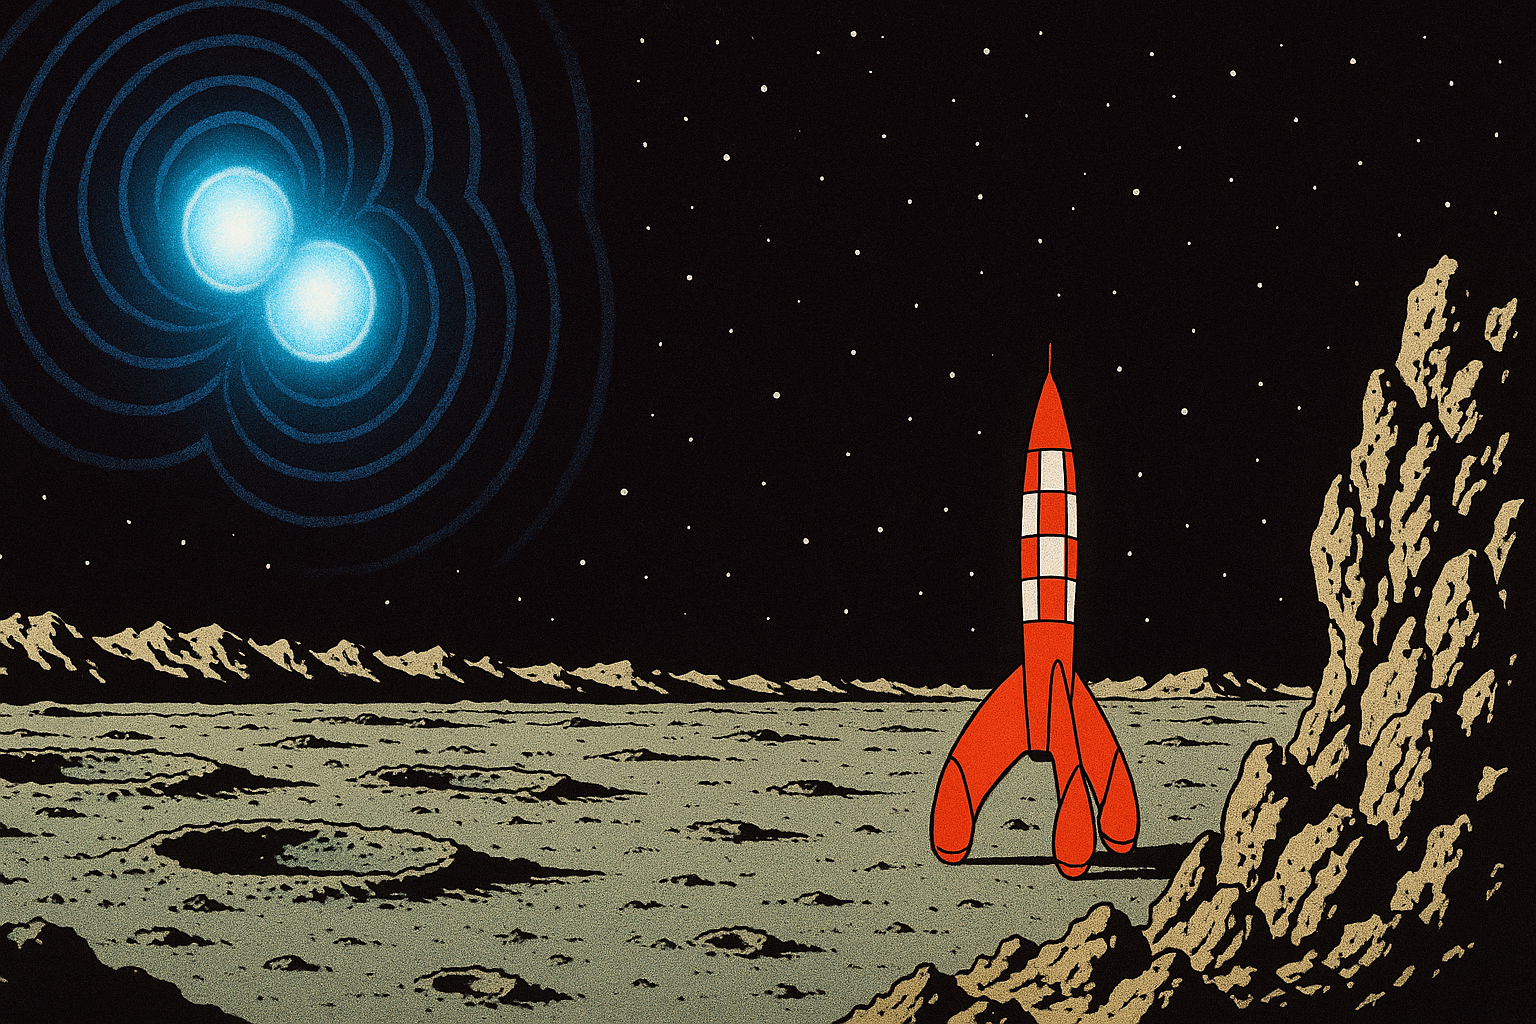
\includegraphics[width=\paperwidth,height=\paperheight]{Figures/tintin_BNS_2.png}}}

\begin{frame}[plain, noframenumbering]

  \begin{tikzpicture}[remember picture,overlay]
    \node[fill=customblue, fill opacity=0.75, text opacity=1, rounded corners=10pt, inner sep=15pt] at (current page.center) {
      \begin{minipage}{0.85\textwidth}
        \centering
        \normalsize\mdseries Scalable and sequential inference of the neutron star equation of state with the Einstein Telescope \\[1.5ex]
        Thibeau Wouters \\[0.5ex]
        \normalsize \github \quad \linkedin \quad \myemail
      \end{minipage}
    };
  \end{tikzpicture}

  \vspace{7cm}

  \begin{columns}
  \column{0.35\textwidth}
  \begin{figure}
    \centering
    \vspace{1.5mm}
    
\includegraphics[width=0.75\linewidth]{Figures/utrecht-university.png}
  \end{figure}
  \column{0.35\textwidth}
  \begin{figure}
    \centering
    
\includegraphics[width=0.75\linewidth]{Figures/Nikhef_logo-transparent.png}
  \end{figure}
\end{columns}

  \end{frame}
}


\begin{frame}{Equation of state inference in the 3G era}
  \def\x{4mm}
  \def\y{2mm}

  \begin{itemize}
    \item Tidal deformations in BNS mergers probe the neutron-star equation of state (EOS)

    \vspace{\x}

    \item Einstein Telescope/Cosmic Explorer: $\mathcal{O}(10^4)$ BNS mergers per year~\smallcite{ET:2019dnz}

    % \vspace{\x}

    % \item Hierarchical inference combines all detections into one EOS posterior

    \vspace{\x}

    \item \red{Bottleneck}: existing methods must restart from scratch as the catalog grows, we need 

    \begin{itemize}
      \vspace{\y}
      \item Scalable: e.g. GPU-acceleration (\textsc{jester})

      \vspace{\y}

      \item \red{Sequential}: reuse previous results, avoid restarting from the prior
    \end{itemize}
  \end{itemize}

  \vspace{\x}

  \begin{tcolorbox}[colback=blue!5!white,colframe=blue!75!black,title=Goal]
    Natural framework for scalable, sequential inference: \blue{sequential Monte Carlo (SMC)}
  \end{tcolorbox}

\end{frame}


% \begin{frame}{Towards scalable, sequential inference}
%   \def\x{4mm}

%   Cost of hierarchical inference grows with the number of sources $N$ — we need:

%   \vspace{\x}

%   \begin{itemize}
%     \item \red{Scalable}: GPU-accelerated hyperlikelihood
%     \begin{itemize}
%       \item Normalizing flows turn single-event posteriors into a tractable hyperlikelihood
%     \end{itemize}

%     \vspace{\x}

%     \item \red{Sequential}: reuse previous results, avoid restarting from the prior

%     \vspace{\x}

%     \item Natural framework: \blue{sequential Monte Carlo (SMC)}
%   \end{itemize}

% \end{frame}


\begin{frame}{Sequential Monte Carlo (SMC)}
  \def\x{4mm}
  \def\y{2mm}

  \begin{itemize}
    \item Particles evolve prior $\rightarrow$ posterior through a sequence of intermediate densities $p_t$: reweight, resample, MCMC move
    
    \vspace{\y}
    
    \item Highly parallelizable: GPU acceleration
    
    \vspace{\y}
    
    \item What choice for sequence $p_t$?
  \end{itemize}

  \vspace{\x}
  \vfill

  \begin{figure}
    \centering
    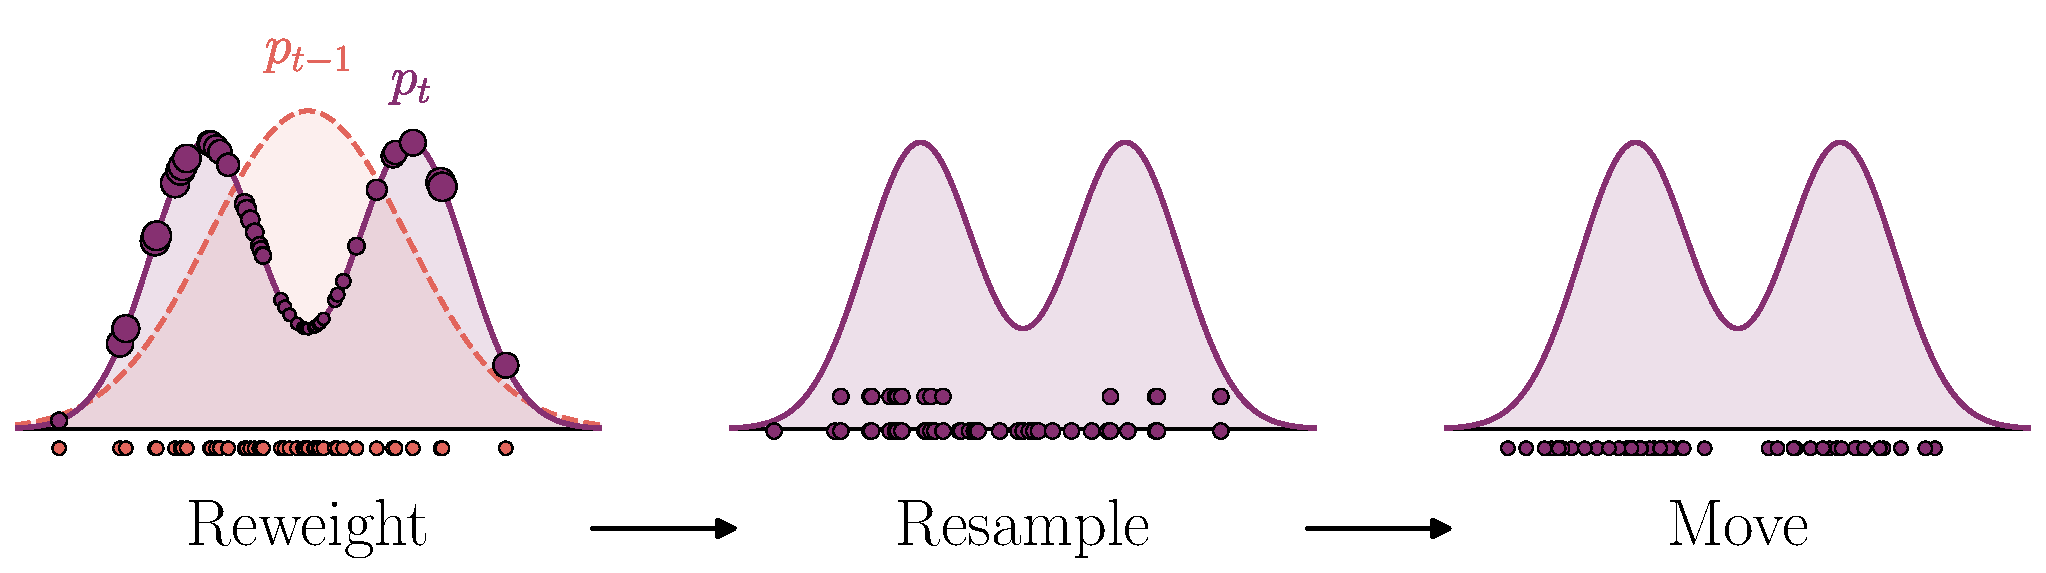
\includegraphics[width=\textwidth]{Figures/smc_steps.pdf}
  \end{figure}

  \vfill

\end{frame}


\begin{frame}{Likelihood vs.\ data tempering}
  \def\x{3mm}
  \def\y{4mm}

  \begin{itemize}
    \item \red{Likelihood tempering}: anneal in the full likelihood, $\mathcal{L}(\theta)^{\beta_t}$, $\beta_t: 0 \rightarrow 1$
    \begin{itemize}
      \item Used in GW PE \tiny (\textsc{pocoMC}~\cite{Karamanis:2022ksp,Williams:2025szm}, \textsc{ASPIRE}~\cite{Williams:2025aar}) \normalsize and \textsc{jester}~\cite{Koehn:2026nin}
    \end{itemize}

    \vspace{\y}

    \item \red{Data tempering}: anneal in new observations one at a time
    \begin{itemize}
      \item Reuse previous posterior
    \end{itemize}
  \end{itemize}

  \vspace{\x}

  \begin{figure}
    \centering
    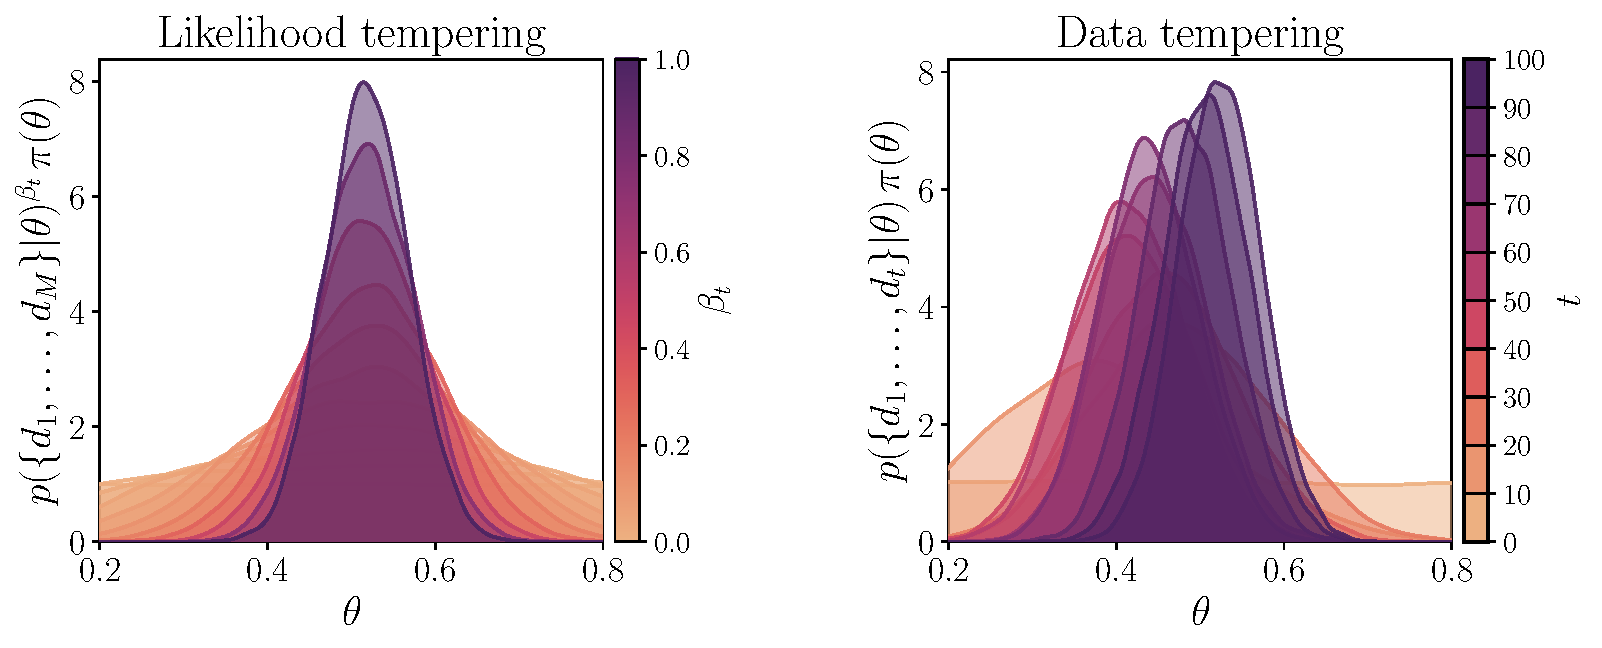
\includegraphics[width=0.95\textwidth]{Figures/smc_temperings.pdf}
  \end{figure}

\end{frame}


\begin{frame}{Adaptive hybrid algorithm}
  \def\x{2mm}

  \begin{itemize}
    \item New events \blue{queued} while effective sample size (ESS) stays high

    \vspace{\x}

    \item ESS drops below threshold $\alpha$ $\Rightarrow$ \red{update} posterior with likelihood tempering over the batch

    \vspace{\x}

    \item Naturally handles \blue{growing catalogs}, without restarting from the prior
  \end{itemize}

  \vspace{5mm}

  \begin{figure}
    \centering
    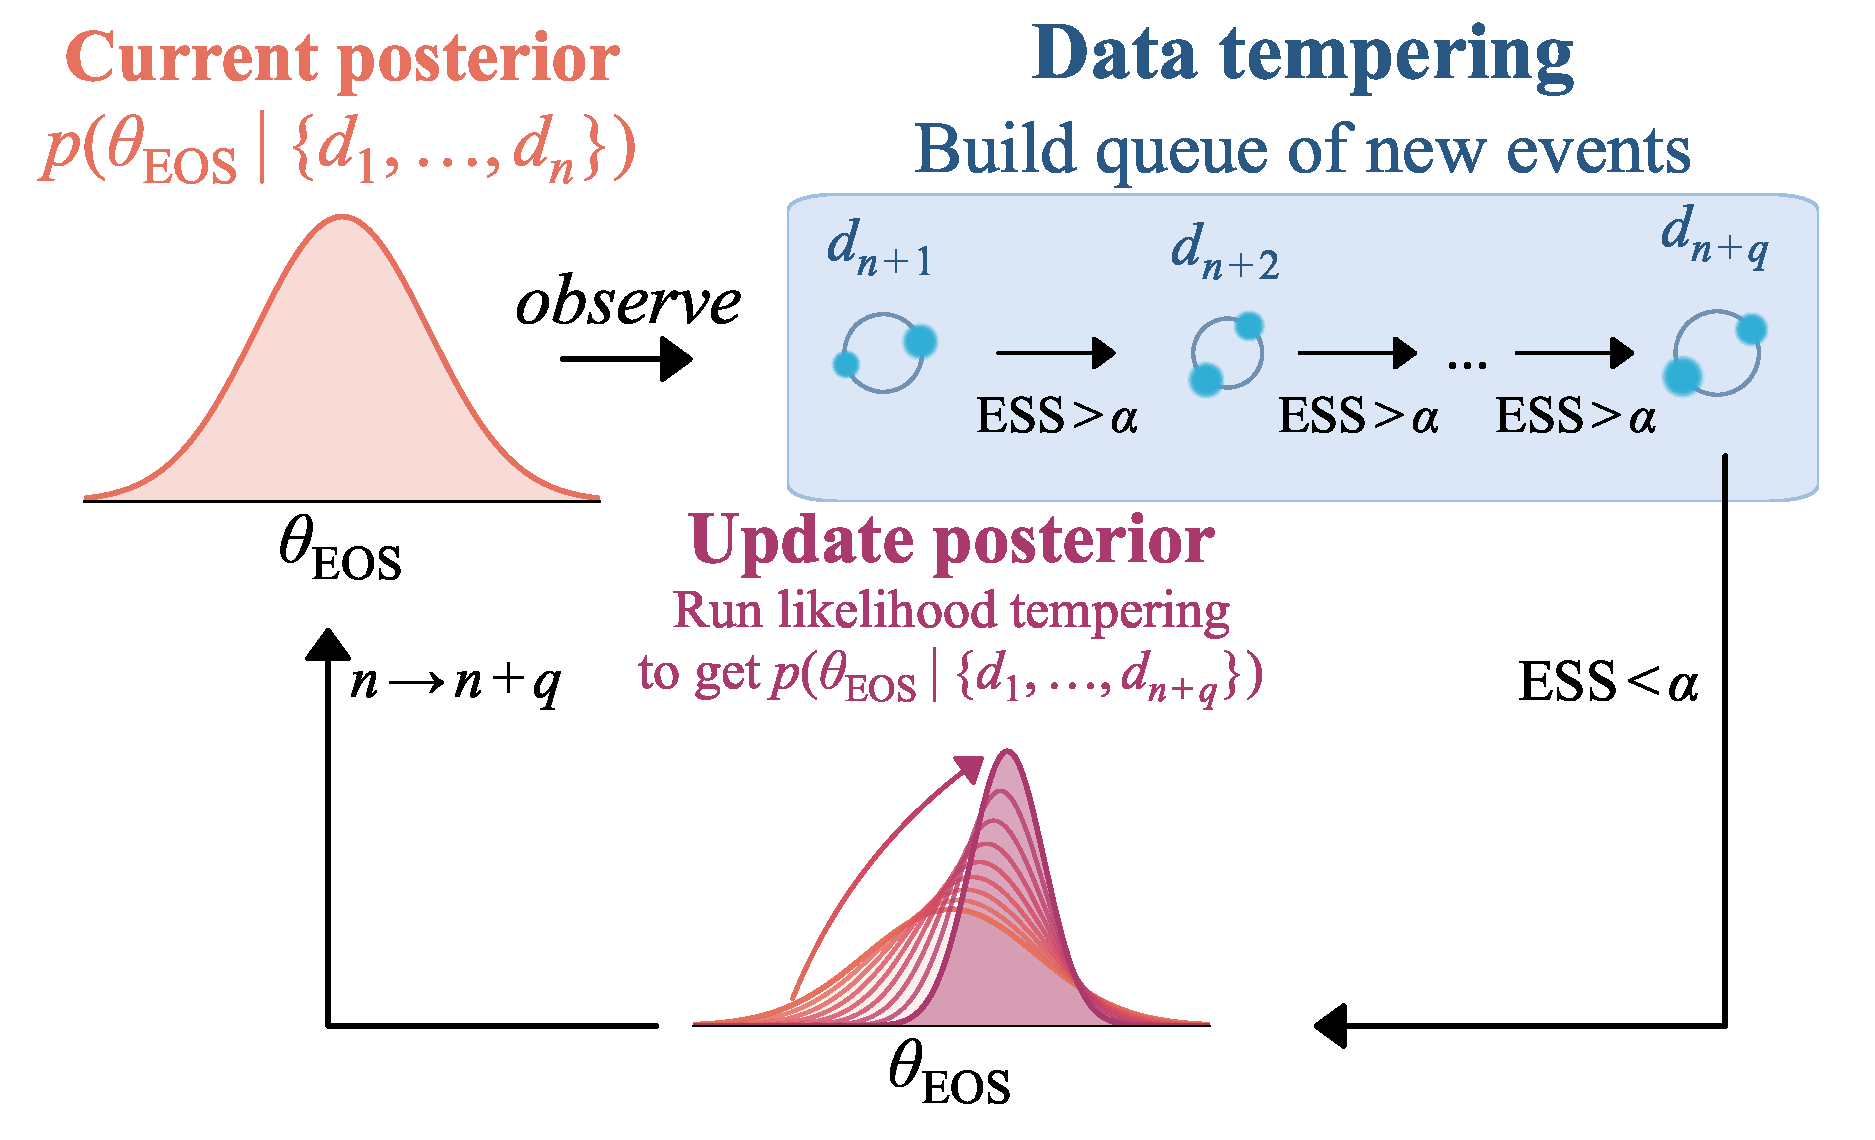
\includegraphics[width=0.68\textwidth]{Figures/fig1_diagram.pdf}
  \end{figure}

\end{frame}


\begin{frame}{Simulating one month of ET data}
  \def\x{3.5mm}

  Demonstrated with proof of concept:

  \vspace{3mm}

  \begin{itemize}
    \item ET 2L-misaligned configuration, Gaussian noise, merger rate $106.6~\mathrm{Gpc}^{-3}\mathrm{yr}^{-1}$

    \vspace{\x}

    \item SNR $>12$ $\Rightarrow$ \red{1555} detected BNS sources in $1$ month

    \vspace{\x}

    \item Single-event PE: nested sampling, masses + tidal deformabilities only, $f_{\mathrm{min}} = 20$~Hz, \texttt{TaylorF2} (simplified settings!)

    \vspace{\x}

    \item \textsc{jester}:
    \begin{itemize}
      \item Sample metamodel + CSE parametrization

      \vspace{2mm}
      
      \item $N = 2000$ SMC particles, ESS threshold $\alpha = 50\%$, prior informed by PSR~J0740+6620~\smallcite{Fonseca:2021wxt}
    \end{itemize}
  \end{itemize}

\end{frame}


\begin{frame}{SMC diagnostics}
  \def\x{3mm}

  \begin{columns}[t]
    \column{0.54\textwidth}
      \begin{figure}
        \centering
        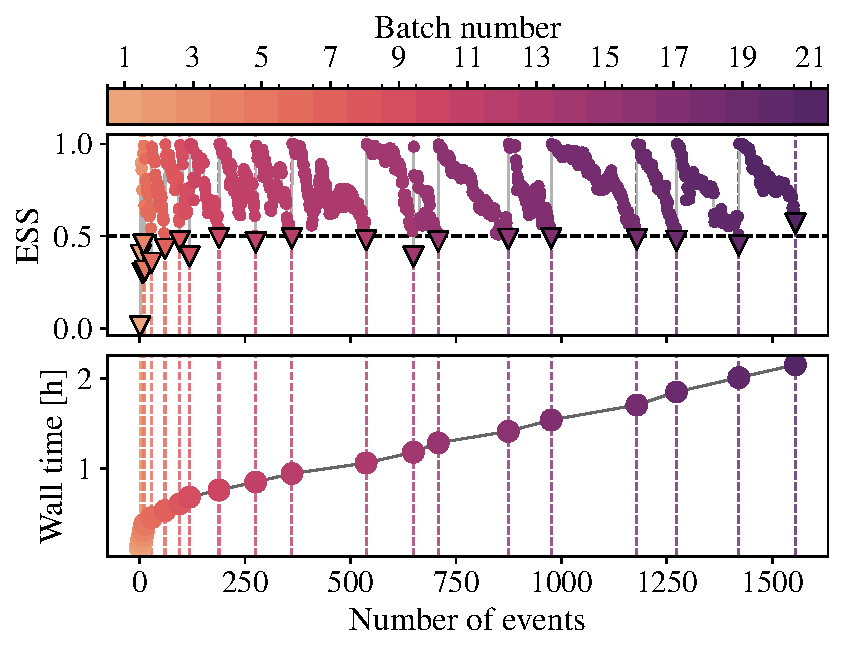
\includegraphics[width=\linewidth]{Figures/fig2_smc_diagnostics_et2l_n1579_noise_time_order.pdf}
      \end{figure}
    \column{0.44\textwidth}
      \begin{itemize}
        \item ESS \red{below 50\%} triggers an update ($\triangledown$)

        \vspace{\x}

        \item Early events highly informative: frequent updates

        \vspace{\x}

        \item Later batches: hundreds of events before the next update

        \vspace{\x}

        \item Total: 22 updates, \red{$\sim 2.2$h} on 1 NVIDIA H100 GPU
      \end{itemize}
  \end{columns}

\end{frame}


\begin{frame}{Equation of state constraints}
  \def\x{3mm}

  \begin{columns}[t]
    \column{0.52\textwidth}
      \begin{figure}
        \centering
        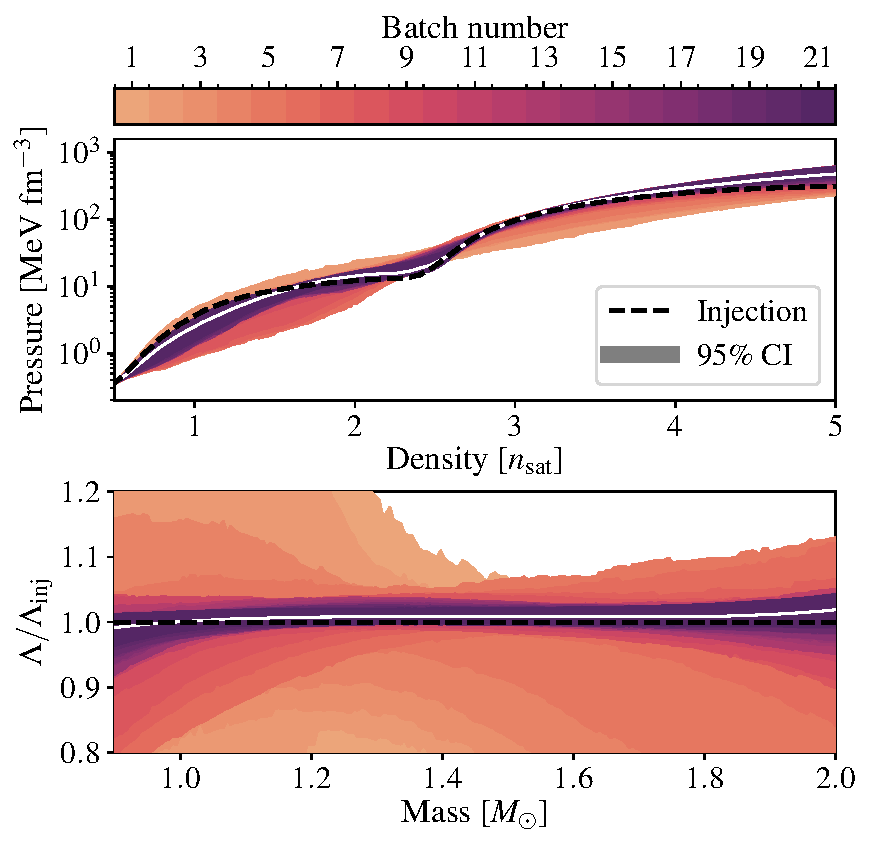
\includegraphics[width=\linewidth]{Figures/fig3_eos_constraints_et2l_n1579_noise_time_order.pdf}
      \end{figure}
    \column{0.46\textwidth}
      \begin{itemize}
        \item Bulk region ($1$--$3\,n_{\rm{sat}}$): pressure under- or overestimated

        \vspace{\x}

        \item Injected $\Lambda$ within the 95\% credible band throughout

        \vspace{\x}

        \item Final batch: $\sim 1\%$ constraints on $\Lambda$ across probed masses
      \end{itemize}
  \end{columns}

\end{frame}


\begin{frame}{Extrapolating to a full year}
  \def\x{1.5mm}

  \begin{figure}
    \centering
    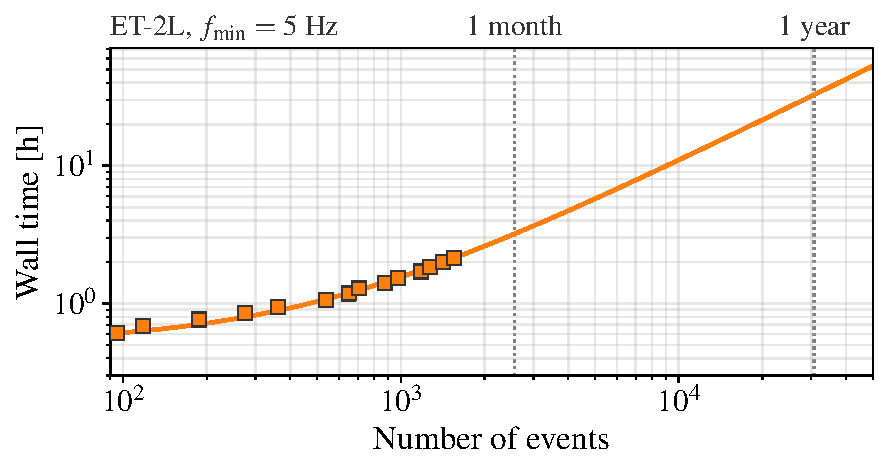
\includegraphics[width=0.65\textwidth]{Figures/fig4_extrap_runtime_projection.pdf}
  \end{figure}

  \vspace{\x}

  \small
  \begin{itemize}
    \item Compute becomes memory-bound $\Rightarrow$ linear fit ($N > 400$)

    \vspace{\x}

    \item More realistic settings ($f_{\rm min} = 5$~Hz): $\sim 2559$ events/month, $\sim 30\,000$/year

    \vspace{\x}

    \item Projected runtime: \red{a few hours} (1 month), \red{$\sim 1.5$ days} (1 year) on a single NVIDIA H100 GPU
  \end{itemize}
  \normalsize

\end{frame}


\begin{frame}{Conclusion \& outlook}
  \def\x{3.5mm}

  \begin{itemize}
    \item Recipe for \blue{scalable}, \red{sequential} hierarchical inference:
    \begin{itemize}
      \item \blue{GPU}: fast hyperlikelihoods
      \item \red{SMC}: data tempering sequentially updates posteriors
    \end{itemize}
    
    \vspace{\x}

    \item Demonstrated on a $\mathcal{O}(10^3)$-event ET mock catalog (nested sampling)

    \vspace{\x}

    \item Extrapolation: a \red{full year} ($\sim 30\,000$ events) feasible within days on a single GPU

    \vspace{\x}

    \item Outlook: joint EOS + population + cosmology inference~\smallcite{Koehn:2026nin}%; flow surrogate for compounded hyperlikelihood cost
  \end{itemize}

\end{frame}


{
\usebackgroundtemplate{\transparent{0.5}{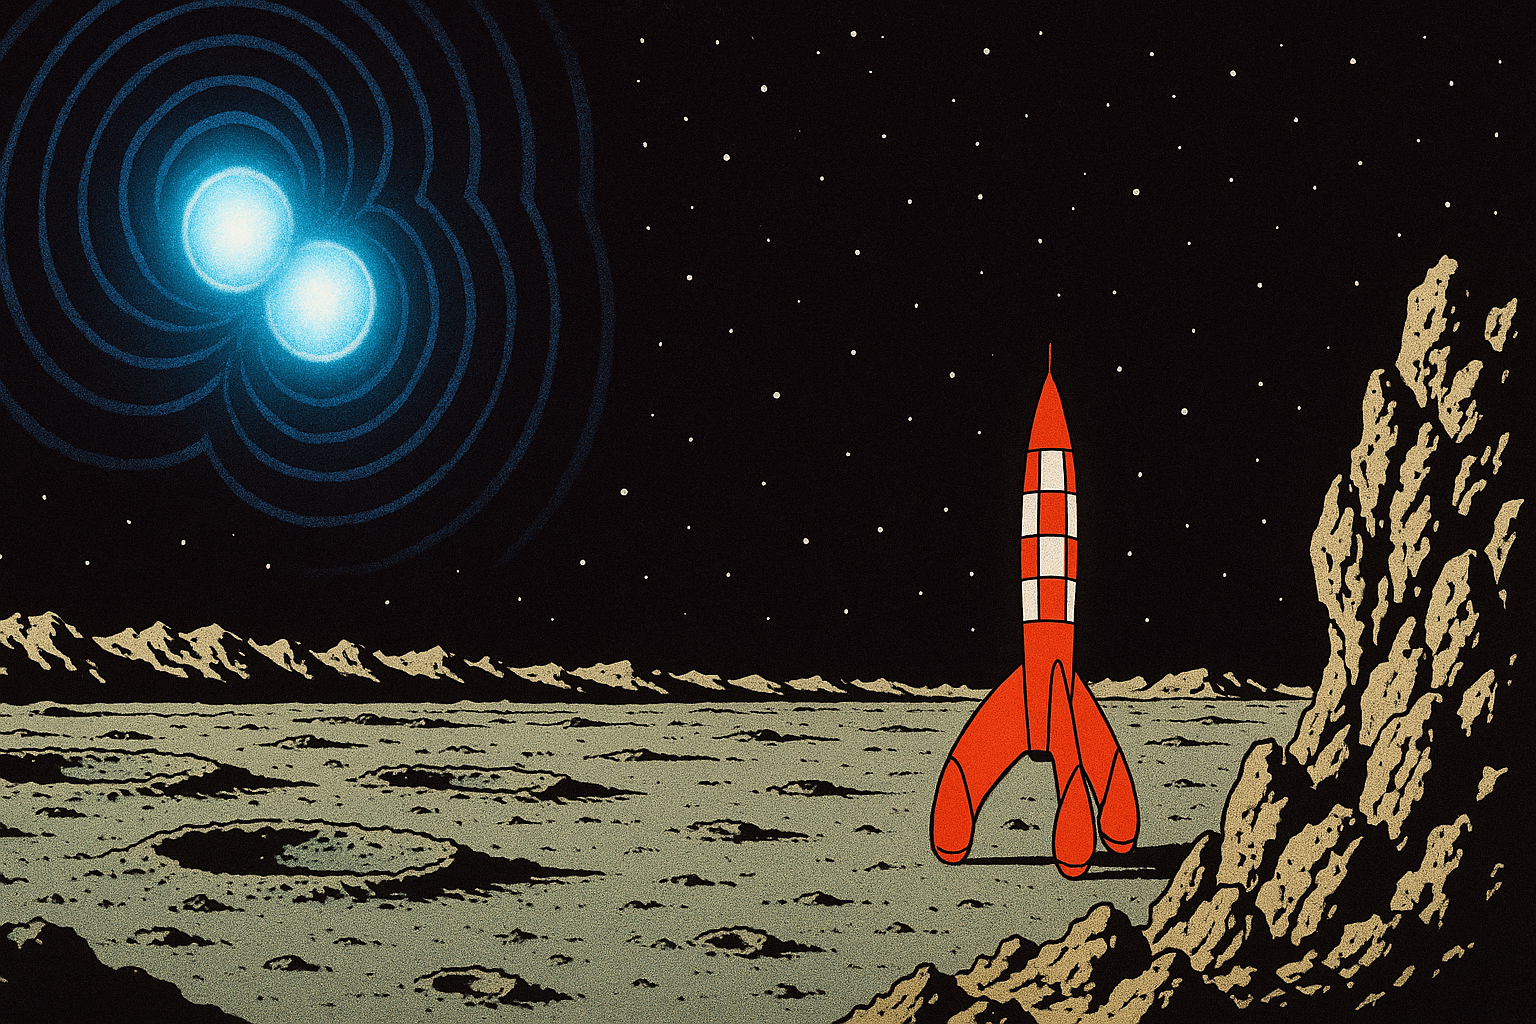
\includegraphics[width=\paperwidth,height=\paperheight]{Figures/tintin_BNS_2.png}}}

\begin{frame}[plain, noframenumbering]

  \begin{tikzpicture}[remember picture,overlay]
    \node[fill=customblue, fill opacity=0.75, text opacity=1, rounded corners=10pt, inner sep=15pt] at ([yshift=2cm]current page.center) {
      \begin{minipage}{0.8\textwidth}
        \centering
        \textbf{Thanks for listening!}
      \end{minipage}
    };
  \end{tikzpicture}

  \end{frame}
}

\begin{frame}[allowframebreaks]{References}
  \printbibliography
\end{frame}

\appendix

% \begin{frame}{Backup: hyperlikelihood \& EOS model}
%   \def\x{2.5mm}

%   \small
%   Hyperposterior over EOS parameters $\thetaeos$:
%   \begin{align*}
%     \mathcal{P}(\thetaeos|\mathcal{D}) &= \frac{\mathcal{L}(\mathcal{D}|\thetaeos)\, \pi(\thetaeos)}{\mathcal{Z}} \, , \\[0.5mm]
%     \mathcal{L}(\mathcal{D}|\thetaeos) &\propto \prod_{i=1}^N \int \frac{p(\theta_i|d_i)}{\pi(\theta_i)}\, p(\theta_i|\thetaeos)\, \diff \theta_i
%   \end{align*}

%   \vspace{-\x}

%   Approximated with a \red{normalizing flow} $q_i$ per event ($M{=}200$ samples):
%   \begin{equation*}
%     \mathcal{L}(\mathcal{D}|\thetaeos) \approx \prod_{i=1}^N \frac1M \sum_{k=1}^M q_i\!\left(m_1^k, m_2^k, \Lambda_{\rm{EOS}}(m_1^k), \Lambda_{\rm{EOS}}(m_2^k)\right)
%   \end{equation*}
%   \normalsize

%   \vspace{\x}

%   \footnotesize
%   EOS model ($D=26$ parameters)~\smallcite{Koehn:2024set}:
%   \begin{itemize}
%     \item Fixed crust below $0.5\,n_{\rm{sat}}$~\smallcite{Douchin:2001sv}
%     \item Metamodel ($\beta$-equilibrium, 4th order)~\smallcite{Margueron:2017eqc}, valid up to $n_{\rm{break}} \in [1,2]\,n_{\rm{sat}}$
%     \item $c_s^2(n)$ extension above $n_{\rm{break}}$: 8 grid points, linear interpolation~\smallcite{Somasundaram:2021clp}
%   \end{itemize}
%   \normalsize

% \end{frame}


\begin{frame}{Backup: SMC --- likelihood tempering}
  \def\x{1mm}

  % \begin{align*}
  %   p_t(\theta) &= \frac{\mathcal{L}(\theta)^{\beta_t}\pi(\theta)}{\mathcal{Z}_t} \, , \quad
  %   w_t^i = \mathcal{L}(\theta_{t-1}^i)^{\beta_t - \beta_{t-1}} \\[0.5mm]
  %   \beta_t &= \sup_{\beta \in [\beta_{t-1},1]}\{\mathrm{ESS}_t(\beta) \geq \alpha N\}
  % \end{align*}

  \small
  \begin{equation*}
    p_t(\theta) = \frac{\mathcal{L}(\theta)^{\beta_t}\pi(\theta)}{\mathcal{Z}_t} \, , \quad \beta_t = \sup_{\beta \in [\beta_{t-1},1]}\{\mathrm{ESS}_t(\beta) \geq \alpha N\}
  \end{equation*}
  \normalsize

  % \vspace{-5mm}
  \vspace{3mm}

  \scriptsize
  \begin{algorithmic}[1]
    \State $t \gets 1$, $\beta_1 \gets 0$, $\hat{\mathcal{Z}}_1 \gets 1$
    \For{$i = 1, \dots, N$}
      \State $\theta_1^i \sim \pi(\theta)$ \Comment{sample from the prior}
    \EndFor
    \While{$\beta_t < 1$}
      \State $t \gets t+1$
      \State $\beta_t \gets \sup_{\beta \in [\beta_{t-1},1]}\{\mathrm{ESS}_t(\beta) \geq \alpha N\}$ \Comment{adaptive temperature}
      \For{$i = 1, \dots, N$}
        \State $w_t^i \gets \mathcal{L}(\theta_{t-1}^i)^{\beta_t - \beta_{t-1}}$ \Comment{reweight}
      \EndFor
      \State $\hat{\mathcal{Z}}_t \gets \hat{\mathcal{Z}}_{t-1} \times \tfrac1N \sum_i w_t^i$ \Comment{update evidence}
      \State resample $\{\theta_{t-1}^i\}$ with weights $\{w_t^i\}$
      \State move particles with MCMC kernel $\mathcal{K}_t$ \Comment{rejuvenation}
    \EndWhile
  \end{algorithmic}
  \normalsize

  \vspace{-1mm}
  \scriptsize Settings: $N=2000$, $\alpha=0.9$, Gaussian random-walk kernel, 20 MCMC steps, target acceptance $0.234$~\smallcite{neal2011optimal}. \normalsize

\end{frame}

\begin{frame}{Backup: SMC --- data tempering}
  \def\x{1mm}

  \small
  \begin{equation*}
    \mathcal{P}_t(\theta) = \frac{\mathcal{L}(d_{1:b_t}|\theta)\pi(\theta)}{\mathcal{Z}_t} \, , \quad b_t = \sup_{b \in [b_{t-1},T]}\{\mathrm{ESS}_t(b) \geq \tilde\alpha N\}
  \end{equation*}
  \normalsize

  % \small
  % \begin{align*}
  %   \mathcal{P}_t(\theta) &= \frac{\mathcal{L}(d_{1:b_t}|\theta)\pi(\theta)}{\mathcal{Z}_t} \, , \quad
  %   w_t^i = \mathcal{L}_{b_{t-1}:b_t}(\theta_{t-1}^i) \\[0.5mm]
  %   b_t &= \sup_{b \in [b_{t-1},T]}\{\mathrm{ESS}_t(b) \geq \tilde\alpha N\}
  % \end{align*}
  % \normalsize

  % \vspace{-4mm}
  \vspace{3mm}

  \scriptsize
  \begin{algorithmic}[1]
    \State $t \gets 0$, $n \gets 0$, $q \gets 0$, $\hat{\mathcal{Z}}_0 \gets 1$
    \For{$i = 1, \dots, N$}
      \State $\theta_0^i \sim \pi(\theta)$, \ $w_0^i \gets 1/N$
    \EndFor
    \While{$t < M$}
      \State $t \gets t+1$, $q \gets q+1$
      \For{$i = 1, \dots, N$}
        \State $w_t^i \gets w_{t-1}^i \times \mathcal{L}_t(\theta_n^i)$ \Comment{reweight with new event}
      \EndFor
      \If{$\mathrm{ESS}_t < \tilde\alpha N$ \textbf{or} $t = M$}
        \State $\{\theta_t^i\}, \hat{\mathcal{Z}}_{n:n+q} \gets$ Alg.~1$(\mathcal{P}_n, \mathcal{L}_{n:n+q})$ \Comment{batch update}
        \State $\hat{\mathcal{Z}}_t \gets \hat{\mathcal{Z}}_n \times \hat{\mathcal{Z}}_{n:n+q}$, \ $n \gets n+q$, \ $q \gets 0$
        \State $w_t^i \gets 1/N$ \Comment{clear the queue}
      \EndIf
    \EndWhile
  \end{algorithmic}
  \normalsize

  \vspace{-1mm}
  \scriptsize Threshold $\tilde\alpha = 0.5$; inner likelihood-tempering step uses the same settings as Algorithm~1. \normalsize

\end{frame}


\begin{frame}{Backup: zero-noise SMC diagnostics}
  \def\x{3mm}

  \begin{columns}[t]
    \column{0.54\textwidth}
      \begin{figure}
        \centering
        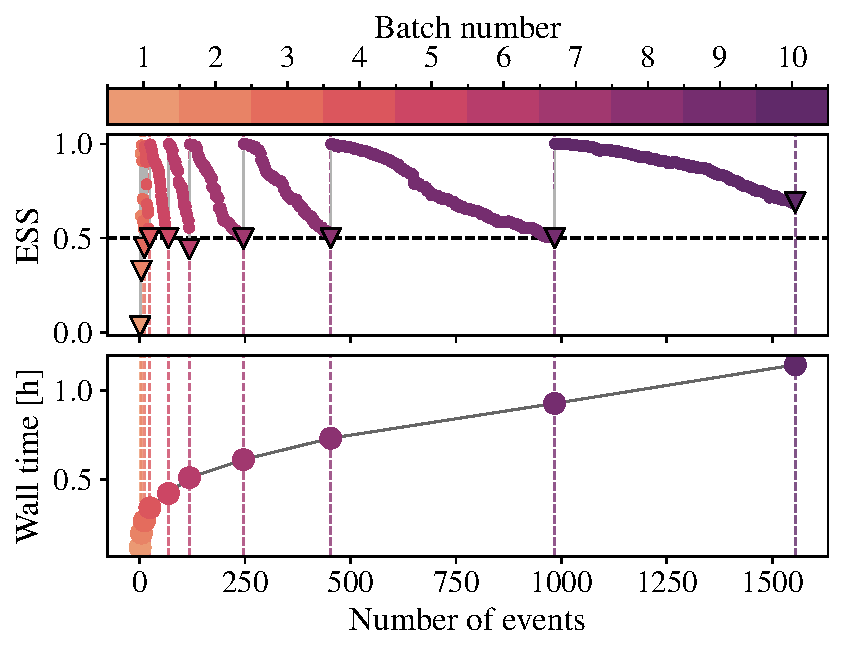
\includegraphics[width=\linewidth]{Figures/fig2_smc_diagnostics_et2l_n1579_time_order.pdf}
      \end{figure}
    \column{0.44\textwidth}
      \begin{itemize}
        \item Same catalog, \red{no detector noise}

        \vspace{\x}

        \item ESS decays smoothly and monotonically, no erratic drops

        \vspace{\x}

        \item Fewer update steps needed: \red{10} batches vs.\ 22 with noise

        \vspace{\x}

        \item Lower total wall time as a result
      \end{itemize}
  \end{columns}

\end{frame}


\begin{frame}{Backup: zero-noise EOS constraints}
  \def\x{3mm}

  \begin{columns}[t]
    \column{0.5\textwidth}
      \begin{figure}
        \centering
        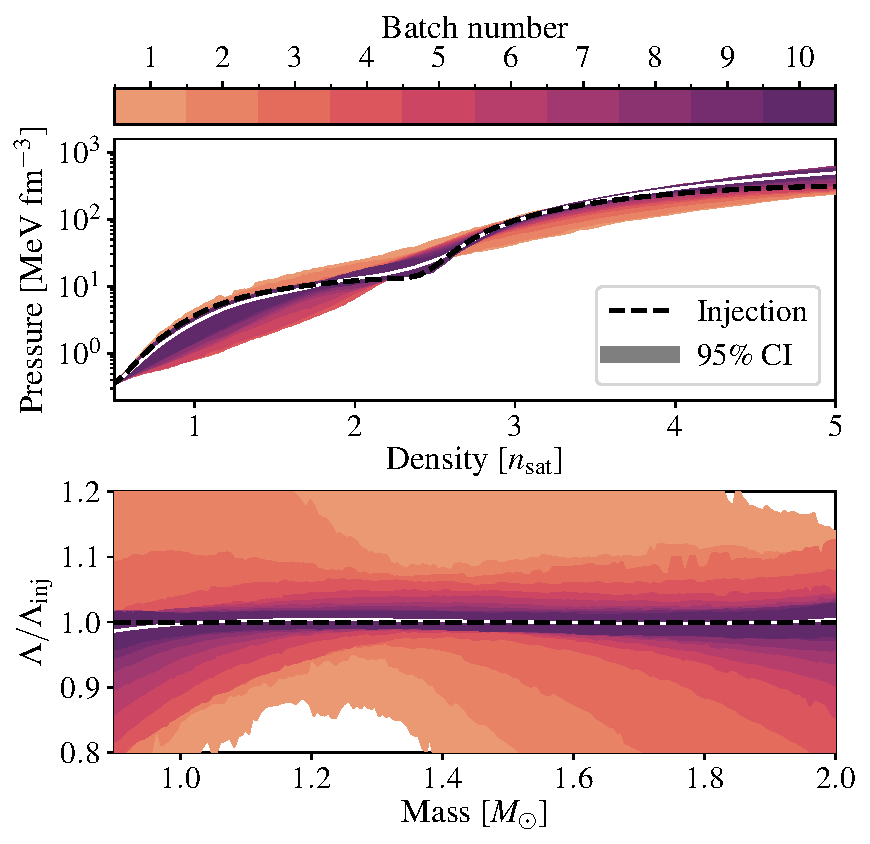
\includegraphics[width=\linewidth]{Figures/fig3_eos_constraints_et2l_n1579_time_order.pdf}
      \end{figure}
    \column{0.48\textwidth}
      \begin{itemize}
        \item Same catalog, \red{no detector noise}

        \vspace{\x}

        \item Median $\Lambda$ curve matches the injection much more closely

        \vspace{\x}

        \item No slight bias in $\Lambda(M)$
      \end{itemize}
  \end{columns}

\end{frame}


% \begin{frame}{Backup: constructing the injected EOS}
%   \def\x{1.5mm}

%   \begin{figure}
%     \centering
%     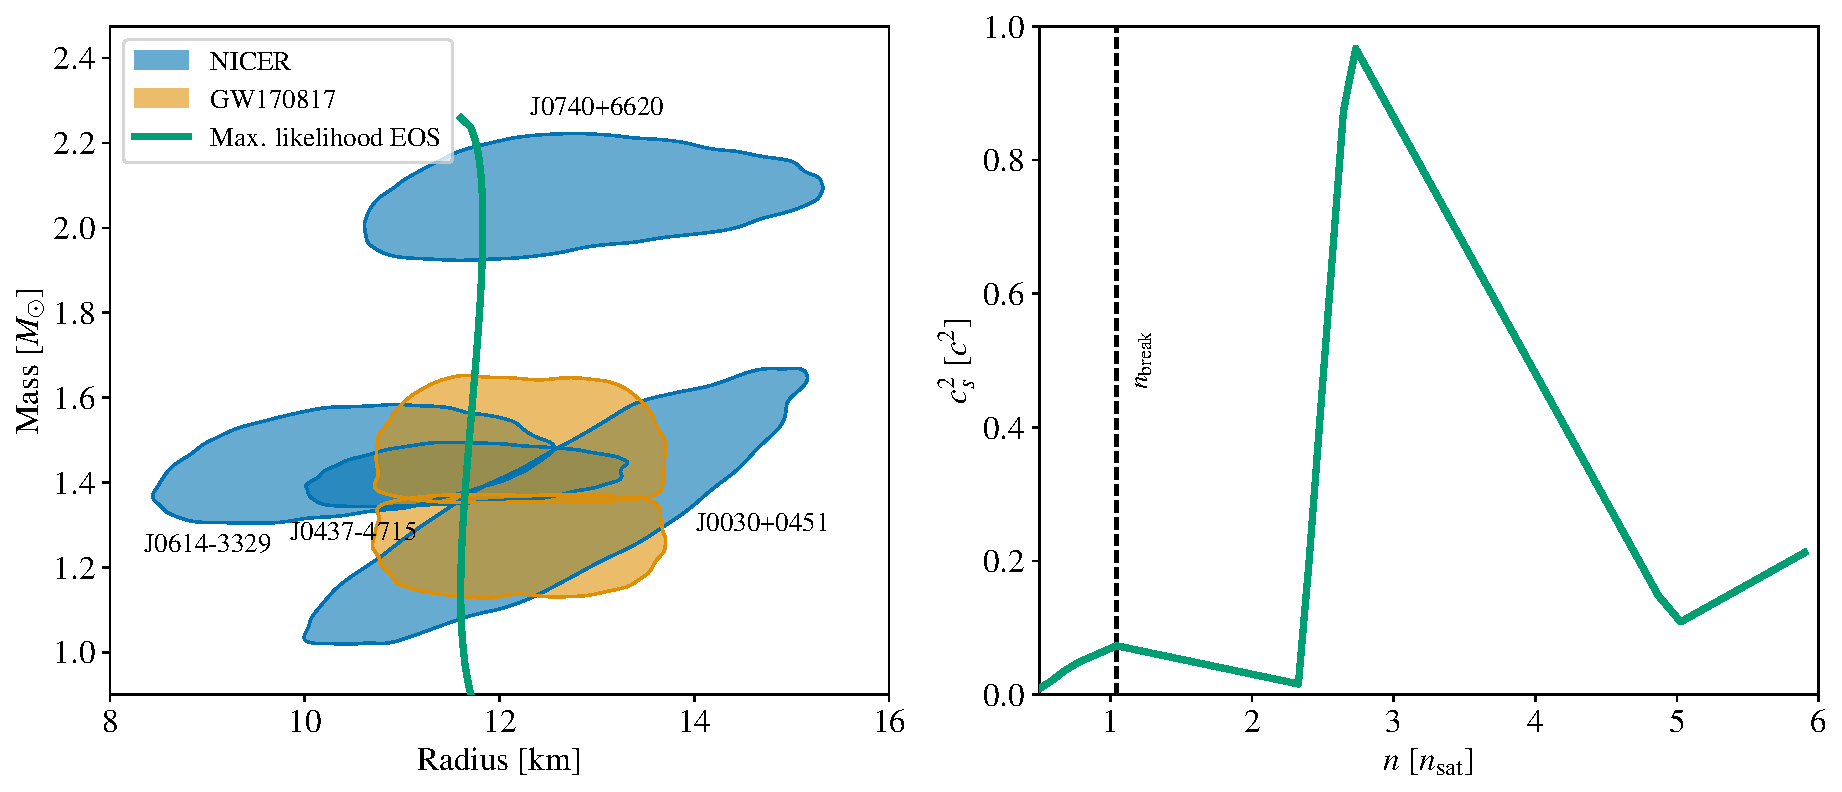
\includegraphics[width=0.68\textwidth]{Figures/app_dataset_mr_cs2.pdf}
%   \end{figure}

%   \vspace{\x}

%   \footnotesize
%   \begin{itemize}
%     \item NICER mass-radius: PSR J0030+0451~\smallcite{Riley:2019yda}, J0740+6620, J0437--4715, J0614--3329

%     \vspace{\x}

%     \item Heavy-pulsar mass: PSR J0740+6620, $(2.08\pm0.07)\,\Msun$~\smallcite{Fonseca:2021wxt}

%     \vspace{\x}

%     \item GW170817 posterior (\texttt{IMRPhenomXP\_NRTidalv3})~\smallcite{Wouters:2025csq}

%     \vspace{\x}

%     \item Injected EOS = \red{maximum-likelihood} \textsc{jester} sample given this combined dataset
%   \end{itemize}
%   \normalsize

% \end{frame}

\end{document}
